

With the continuum framework established, the constitutive equations defined, and the material parameters identified, this section addresses the numerical verification and application of the developed formulation. The non-linear weak form and finite element framework detailed in Section \ref{sec:FEM residuals} are deployed to simulate a series of representative multi-field initial-boundary value problems (IBVPs).

\subsection{Numerical verification and mesh convergence of pre-stretched dielectric elastomers: a circular-equivalent membrane benchmark}

The primary technical objectives of this numerical example are:

\begin{enumerate}
    \item To verify the algorithmic robustness, stability of the proposed Total Lagrangian Finite Element (FEM) formulation under coupled thermoelectromechanical loading, finite strain and pre-stretched conditions.
    \item To perform a mesh convergence study to evaluate the spatial discretization sensitivity and ensure mesh-independent stress and displacement fields.
    \item To assess the performance of the calibrated thermo-electro-mechanical constitutive model under different long-term hyper-elastic components.
    \item To benchmark the numerical results (e.g., radial stretch $\lambda_1$ and out-of-plane displacement) against established analytical solutions or experimental data available in the literature.
\end{enumerate}


\begin{figure}[htp]
    \centering
    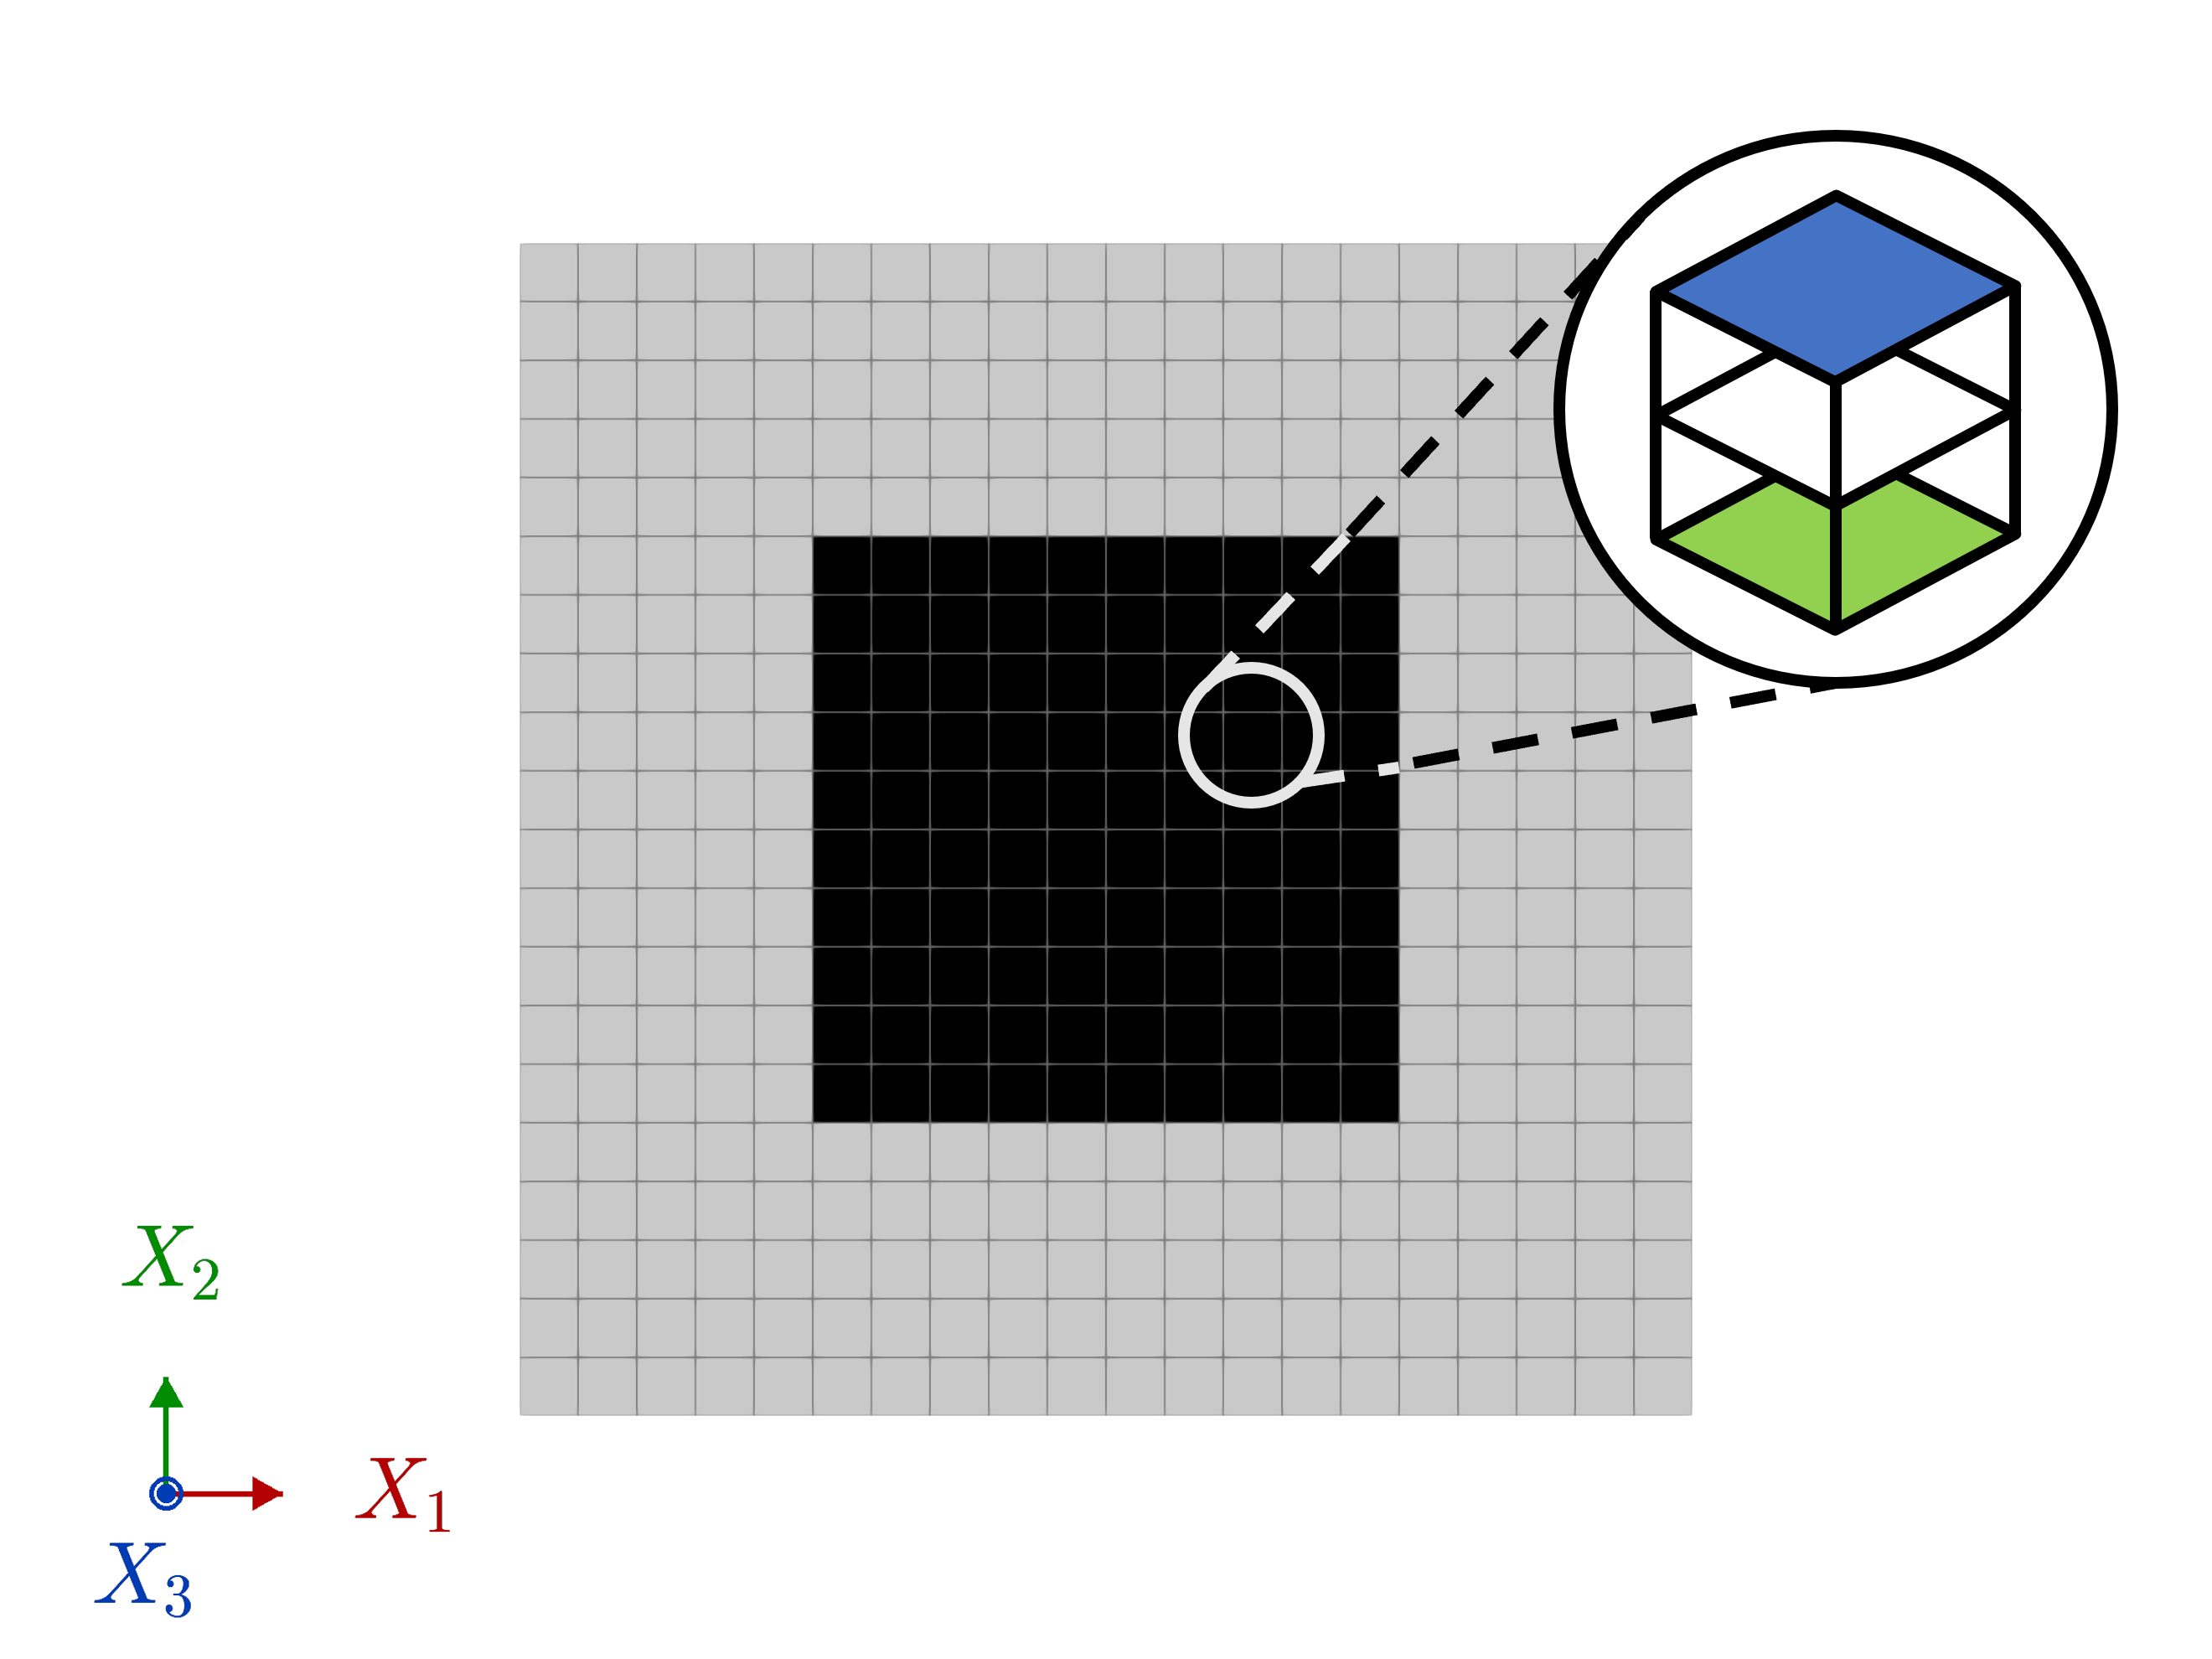
\includegraphics[width=.6\textwidth]{figures/membrane/membrane_geometry.png}
    \caption{Geometry of the dielectric membrane and discrete model. The black region corresponds to the top electrode.}
    \label{fig:membrane_geometry}
\end{figure}


\begin{table}[htp]
    \centering
    \caption{Geometry and parameters}
    \label{tab::membrane_parameters}
    \begin{tabular}{lc}
        \toprule
        Frame width & \qty{5}{\cm} \\
        Undeformed thickness & \qty{1}{\mm} \\
        Maximum voltage & \qty{10}{\kV} \\
        Prestretch $\lambda_p$ & 1-3 \\
        Reference temperature $\theta_R$ & \qty{20}{\celsius} \\
        Material & VHB4910 (section \ref{sec:calibration}) \\
        \bottomrule
    \end{tabular}
\end{table}



\begin{figure}
    \centering
    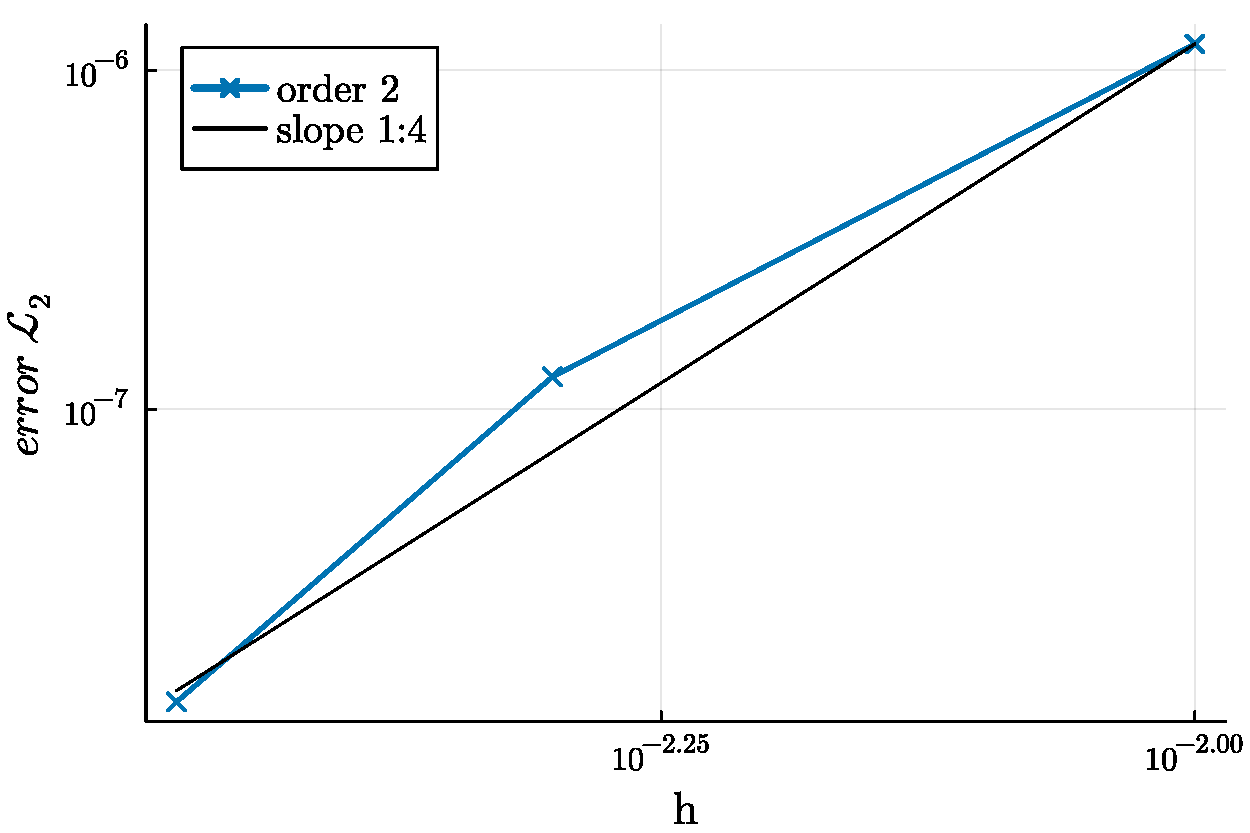
\includegraphics[width=.6\textwidth]{figures/membrane/convergence.pdf}
    \caption{Mesh convergence analysis. $\mathcal{L}_2$ norm error of the displacement field.}
    \label{fig:membrane_convergence}
\end{figure}



\begin{figure}[htp]
    \centering
    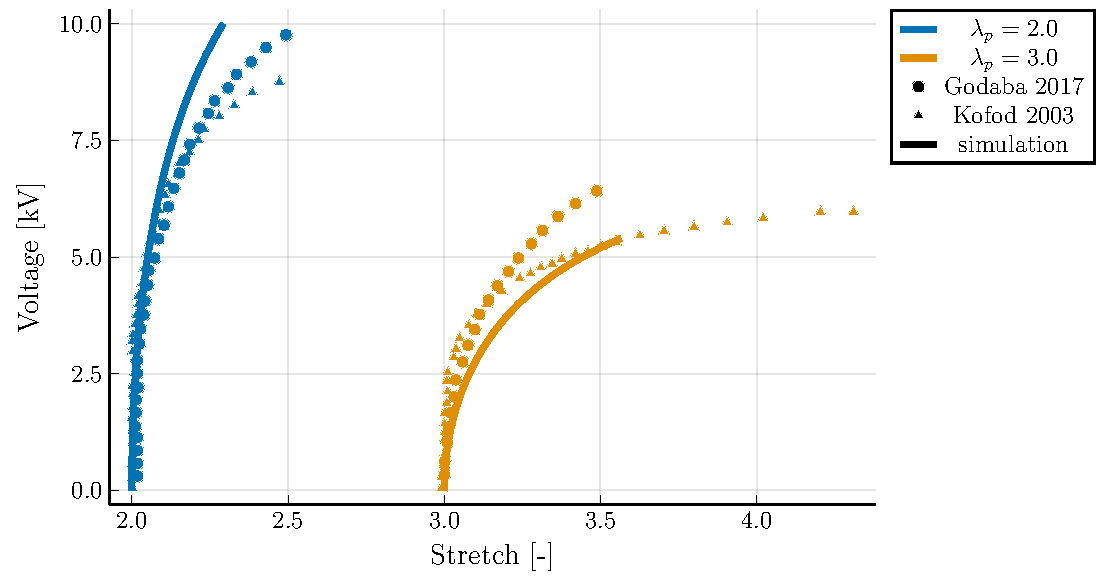
\includegraphics[width=.6\textwidth]{figures/membrane/stretch_voltage_comparison.pdf}
    \caption{Comparison of the results of a FEM simulation using the current constitutive model and different experimental data reported in the literature.}
    \label{fig:literature_comparison}
\end{figure}
